\documentclass[12pt]{beamer}

\usetheme{Warsaw}
\useoutertheme{split}
\useinnertheme{circles}
\usecolortheme{crane}

\usepackage{polski}
\usepackage[utf8]{inputenc}
\usepackage[english,polish]{babel}

\usepackage{xcolor}
\definecolor{default_color}{RGB}{0,0,0}
\colorlet{dcolor}{default_color}
\setbeamercolor{title}{fg=dcolor}
\setbeamercolor{titlelike}{fg=dcolor}
\setbeamercolor{frametitle}{fg=dcolor}

\usepackage{listings}
\lstdefinestyle{customcpp}{
  belowcaptionskip=1\baselineskip,
  breaklines=true,
  frame=L,
  xleftmargin=\parindent,
  language=C++,
  showstringspaces=false,
  basicstyle=\fontsize{9pt}{9}\ttfamily,
  keywordstyle=\bfseries\color{green!40!black},
  commentstyle=\itshape\color{purple!40!black},
  stringstyle=\color{orange},
}
\lstset{
	backgroundcolor=\color{white},
	language=C++,
	style=customcpp,
	tabsize=2
}


\usepackage{enumerate}
\setbeamertemplate{enumerate item}{$\textcolor{dcolor}{\insertenumlabel.}$}
\setbeamertemplate{enumerate subitem}{$\textcolor{dcolor}{\insertenumlabel.\insertsubenumlabel.}$}
\setbeamertemplate{enumerate subsubitem}{$\textcolor{dcolor}{\insertenumlabel.\insertsubenumlabel.\insertsubsubenumlabel.}$}

\setbeamertemplate{itemize item}{$\textcolor{dcolor}-$}
\setbeamertemplate{itemize subitem}{$\textcolor{dcolor}\bullet$}
\setbeamertemplate{itemize subsubitem}{$\textcolor{dcolor}\triangleright$}

\usepackage{tikz}
% \usebackgroundtemplate{
% 	\tikz[overlay,remember picture]\node[opacity=0.4]at (current page.center){
% 		% source: https://upload.wikimedia.org/wikipedia/commons/thumb/1/18/ISO_C%2B%2B_Logo.svg/1822px-ISO_C%2B%2B_Logo.svg.png
% 		
\includegraphics[width=4cm]{cpp_logo.png}
% 	};
% }

\subtitle{Implementacja i~badanie wydajności serializacji wykonanej w~paradygmacie metaprogramowania względem standardowych rozwiązań w~języku C++}
\title{Omówienie pracy magisterskiej}
\author[inż. Krzysztof Mochocki]{inż. Krzysztof Mochocki}
\date{}


\begin{document}

	\begin{frame}
		\centering
\includegraphics[width=0.2137\framewidth, keepaspectratio=true]{../paper/img/black_and_wtransparent_polsl_horizontal_logo.png}
		\maketitle
	\end{frame}

	\begin{frame}
		\frametitle{Wstęp}
		\begin{enumerate}
			\item Dostępne rozwiązania
			\begin{enumerate}
				\item Przykładowa hierarchia klas
				\item Manualna refleksja
				\item Pół automatyczna refleksja
			\end{enumerate}
			\item Zaproponowane rozwiązanie
			\item Badanie
			\begin{enumerate}
				\item Środowisko testowe
				\item Uzyskane wyniki
			\end{enumerate}
			\item Wnioski
		\end{enumerate}
	\end{frame}

	\begin{frame}
		\frametitle{Dostępne rozwiązania: przykładowa hierarchia klas}

		\begin{figure}[ht!]
			\centering
			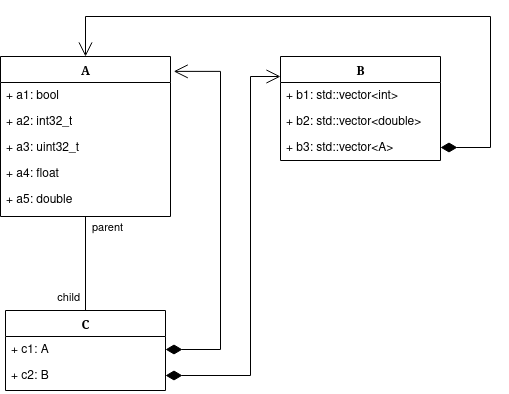
\includegraphics[width=0.75\framewidth, keepaspectratio=true]{../paper/img/benchmark_model_uml_diagram.png}
			\caption{Diagram UML reflektowanej klasy}
		\end{figure}

	\end{frame}

	\begin{frame}[fragile]
		\frametitle{Dostępne rozwiązania: manualne}

		Manualna serializacja wspomagana przez zewnętrzną bibliotekę

		\begin{lstlisting}[frame=single]
json["b1"] = Json::Value(Json::ValueType::arrayValue);
json["b1"].resize(in.b1.size());
for(const auto& it: in.b1) json["b1"].append(it);

json["b2"] = Json::Value(Json::ValueType::arrayValue);
json["b2"].resize(in.b2.size());
for(const auto& it: in.b2) json["b2"].append(it);

json["b3"] = Json::Value(Json::ValueType::arrayValue);
json["b3"].resize(in.b3.size());
for(const auto& it: in.b3)
{
	Json::Value it_result;
	serial_A(it_result, it);
	json["b3"].append(it_result);
}
		\end{lstlisting}

	\end{frame}

	\begin{frame}[fragile]
		\frametitle{Dostępne rozwiązania: pół automatyczne}

		Automatyczna serializacja z manualną refleksją pól

		\begin{lstlisting}[frame=single]
// plik naglowkowy
FC_REFLECT(fc_model_t::A, (a1)(a2)(a3)(a4)(a5));
FC_REFLECT(fc_model_t::B, (b1)(b2)(b3));
FC_REFLECT_DERIVED(fc_model_t::C, (fc_model_t::A), (c1)(c2));

// plik zrodlowy
void serialize(const model_t& in, std::string& out) const
{
	fc::mutable_variant_object mvo{};
	fc::reflector<model_t>::visit(
		fc::to_variant_visitor<model_t>(
			mvo, in, 10
		)
	);
	out = fc::json::to_string(mvo);
}
		\end{lstlisting}

	\end{frame}

	\begin{frame}[fragile]
		\frametitle{Zaproponowane rozwiązanie: w pełni automatyczne}

		Automatyczna serializacja z automatyczną refleksją pól

		\begin{lstlisting}[frame=single]
struct A_impl
{
	serek::ffield<bool> a1{};
	serek::field<&A_impl::a1, int32_t> a2{};
	serek::field<&A_impl::a2, uint32_t> a3{};
	serek::field<&A_impl::a3, float> a4{};
	serek::field<&A_impl::a4, double> a5{};
};
using A = serek::pack<&A_impl::a5>;

struct C_impl : public A_impl
{
	serek::field<&C_impl::a5, A> c1{};
	serek::field<&C_impl::c1, B> c2{};
};
using C = serek::pack<&C_impl::c2>;
		\end{lstlisting}

	\end{frame}

	\begin{frame}
		\frametitle{Badania: wykorzystane technologie}

		\begin{enumerate}
			\item Python
			\begin{itemize}
				\item generowanie danych
				\item obrabianie wyników
				\item generowanie wykresów
			\end{itemize}
			\item Apache JMeter\texttrademark
			\begin{itemize}
				\item projektowanie testów wydajnościowych
				\item generowanie wstępnych raportów
				\item testowanie konfiguracji
				\item uruchamianie testów
			\end{itemize}
			\item HTTP Framework Drogon CPP
			\begin{itemize}
				\item stworzenie środowiska, w którym biblioteki były testowane
				\item zapewnienie interfejsu do testowani
			\end{itemize}
		\end{enumerate}
	\end{frame}

	\begin{frame}
		\frametitle{Badania: przepustowość}

		\begin{figure}[ht!]
			\centering
			\includegraphics[width=\framewidth, keepaspectratio=true]{../paper/charts/output_with_charts_as_images/throughput_per_library.png}
			\caption{Przebieg przepustowości w funkcji sekundy trwania testu}
		\end{figure}

	\end{frame}

	\begin{frame}
		\frametitle{Badania: sumaryczny rozkład czasów}

		\begin{figure}[ht!]
			\centering
			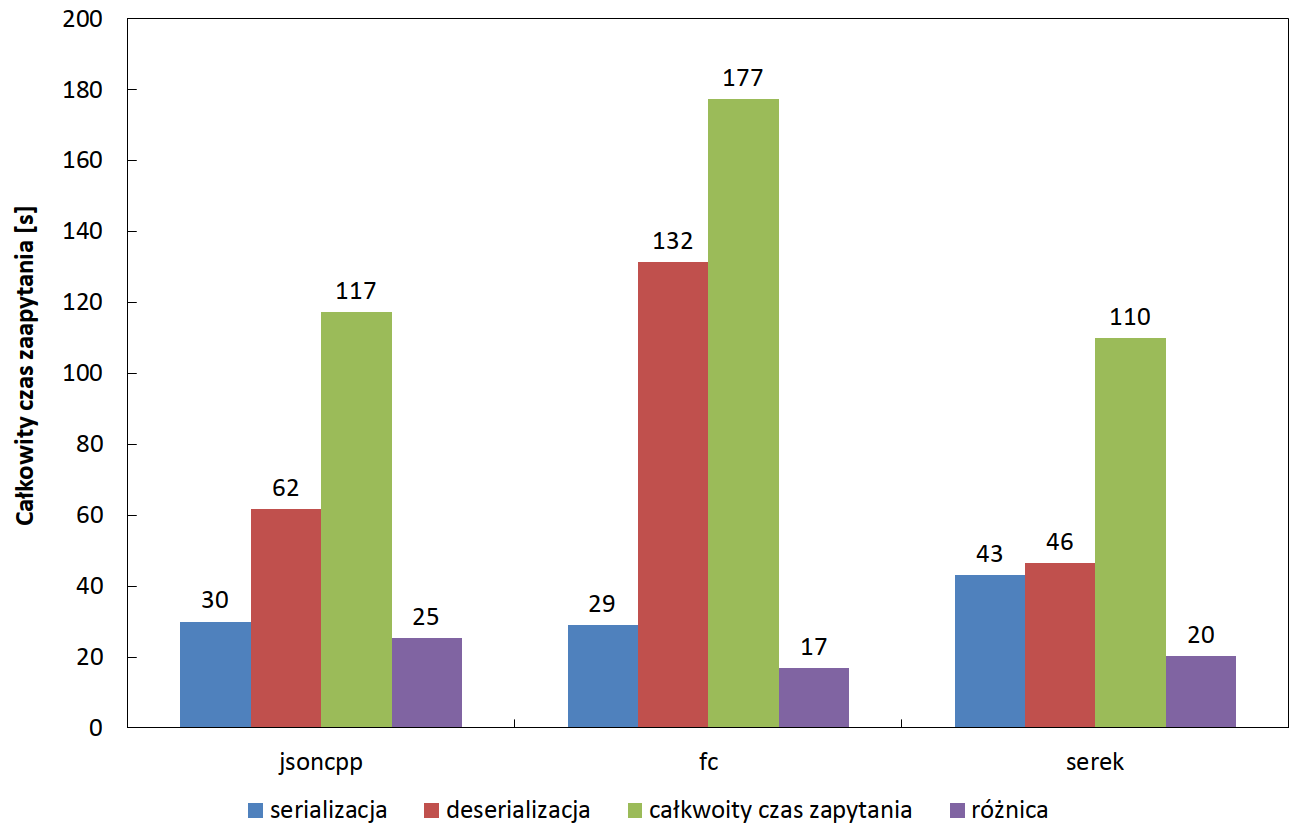
\includegraphics[width=\framewidth, keepaspectratio=true]{../paper/charts/pre_generated_charts/total_serial_and_deserial_library_summmary.png}
			\caption{Sumaryczny rozkład czasu podczas badania}
		\end{figure}

	\end{frame}

	\begin{frame}
		\frametitle{Wnioski}

		\begin{itemize}
			\item Ogólnie najszybszą biblioteką okazała się eksperymentalna
			\item Jednocześnie będąc najwolniejszą w serializacji i najszybszą w deserializacji
			\item Został zaobserwowany brak stabilności w przepustowości biblioteki $serek$
		\end{itemize}

	\end{frame}

	\begin{frame}
		\frametitle{Koniec}

		\centering\Huge Dziękuje za uwagę!

	\end{frame}

\end{document}
